\documentclass{article}
\usepackage{graphicx} 
\usepackage[dutch]{babel}
\usepackage{graphicx}
\graphicspath{ {./images/} }
\begin{document}
\sffamily



\begin{titlepage}
  \centering
    \vfill
    {\bfseries\Huge
      Individueel Verslag Tinlab Advanced Algorithms \\
        \vskip2cm
      }
      {\bfseries\Large
        Jordi Luijk\\
      }
      {
        \bfseries\normalsize
        0889529\\
        \vskip1cm
        \today\\
    }    
    \vfill
    
\includegraphics[width=4cm]{logohr.png} % also works with logo.pdf
    \vfill
    \vfill
\end{titlepage}
\newpage
\tableofcontents

\newpage
\section{Inleiding}
In dit document wordt samengevat uitleg, voorbeelden en uitwerkingen van oefeningen beschreven. Deze samenvatting dient als leerboekje waar naar gerefereerd kan worden. 


royce waterfall method






World vs. machine:



4 variablen methode:


Mode confusion 
%\cite{bredereke2002rigorous}, //geeft definitie van mode confusion.




\section{Case study}
Hieronder staan case studies beschreven die de verschillende principes van dit document demonstreren.

\subsection{Kanon met dubbele loop van John Gilleland}
\subsubsection{Achtergrond}
Het kanon met dubbele loop is een mislukt experimenteel wapen ontwikkeld in de 19e eeuw. Het idee achter het wapen was om twee kanonskogels te verbinden met ketting en iedere kanonskogel in zijn eigen loop te laden. Het concept van verbonden kanonskogels bestond al, deze ketting shotten werden gebruikt in een kanon met één loop om masten van schepen te verwoesten. De innovatie zat hem in de dubbele loop en er werd verwacht dat dit effectief zou zijn in het neermaaien van soldaten.
\subsubsection{Wat ging er mis?}
De lopen vuren niet tegelijkertijd. Hierdoor zijn de kanonskogels heel irregulier in waar zijn naartoe gaan. Het zet ook veel stress op de ketting waardoor deze kan breken.
\subsubsection{Modellen}
Met het gebruik van de modellen in hoofdstuk \ref{SoortenModellen}, zien we dat het probleem niet uit de buitenwereld komt maar binnen het systeem zelf plaatsvindt. In het vier variabelen model zou het kanon een probleem hebben in de actuatoren.

\subsection{Nucleaire testen op het eiland Bikini Atoll}
\subsubsection{Achtergrond}
Nucleaire bom testen werden gehouden op het eiland Bikini Atoll. Een van deze bommen is had een explosie van 15 megaton in plaats van de verwachte 4-8 megaton.
\subsubsection{Wat ging er mis?}
Uitgaande van de bestaande kennis van fysica van de tijd had de bom een verwachte lading van 6 megaton moeten bedragen. Dat de kennis incompleet was werd duidelijk toen de daadwerkelijke explosie meer dan twee zo hoog was.
\subsubsection{Modellen}
Met het gebruik van de modellen in hoofdstuk \ref{SoortenModellen}, zien we dat het probleem niet uit de buitenwereld komt maar binnen het systeem zelf plaatsvond. Er was een onverwachte reactie in de lithium in het systeem \cite{castlebravonuke}.

\section{Research}

\subsection{Mode Confusion}
Systemen hebben bepaalde staten waarin zei zich kunnen bevinden en een gebruiker heeft een mentaal model hiervan. Wanneer het mentale model en de tekens die het systeem afgeeft niet meer in sync zijn dan spreken we van 'mode confusion' \cite{bredereke2002rigorous}. Dit fenomeen kan gevaarlijke gevolgen hebben.

\section{Requirements}

In dit hoofdstuk wordt er over requirements en specificaties aangeduid. De definities voor deze termen zijn die in dit document zullen worden aangehouden zijn die van \cite{thompson2000requirements}. \newline

\subsection{Requirements}

Requirements beschrijven fenomenen uit de buitenwereld die een probleem beschrijven. \newline \newline
Licht, temperatuur, mensen en andere al bestaande systemen zijn allemaal voorbeelden van fenomenen die door requirements beschreven kunnen worden. \newline

Mogelijke methode voor het vaststellen van requirements zijn: \newline
- vragen stellen / enquête \newline
- observeren \newline
- brainstormen \newline
- ervaring / literatuurstudie \newline
- specialist raadplegen \newline


\subsection{specificaties}

Specificaties zijn de eisen waaraan de oplossing of product aan moet voldoen en mee wordt geëvalueerd. Software en hardware zijn voorbeelden van specificaties.

\section{Modellen}

\subsection{De Kripke structuur}

Kripke structuren zijn een manier om het gedrag van een systeem te modelleren. Belangrijke termen voor het bespreken van Kripke structuren zijn states en transities. \newline

Een state beschrijft de toestand waarin een systeem zich bevindt. In het geval dat de state niet duidelijk is voor de gebruiker dan wordt dat mode confusion genoemd. Transities zijn de overgangen van één state naar de anderen. 

\begin{figure}[!h]
	\centering
	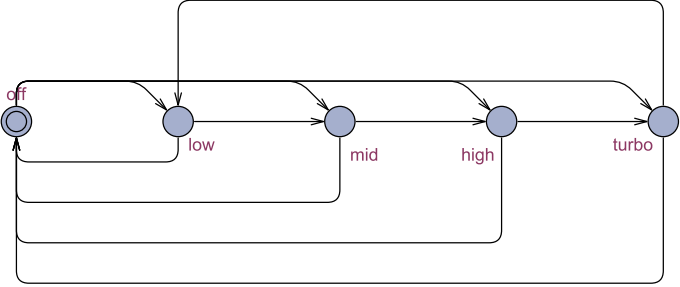
\includegraphics[width=\textwidth]{kripke_structure_example1}
    \caption{Voorbeeld Kripke structuur}
	%\label{fig:figure2}
\end{figure}

\subsection{Soorten modellen} \label{SoortenModellen}

\textbf{World vs. machine:} 

Er kan onderscheid worden gemaakt tussen de fenomenen die zich bevinden in de wereld buiten het systeem en de fenomenen die alleen in het systeem zelf bestaan. \newline
\textbf{4 variabelen methode:}

Modellen voor computer systemen gebruiken vaak antropomorfisme analogie en intuïtieve conclusies wat tot lager precisie kan leiden. Het vier variabelen model helpt om software vereisten met groter precisie vast te stellen, door deze te modelleren op een manier zoals vaak door ingenieurs wordt toegepast. \cite{parnas1995functional} 

Zoals de naam suggereert bestaat het vier variabelen model uit vier onderdelen. Input, output, gecontroleerde variabelen en gemonitorde variabelen. Als eerste de gemonteerde variabelen die buiten het systeem bestaan en worden opgenomen door sensoren, waarna deze input is voor de software. Deze input draagt bij aan de output of acties die het systeem in de buitenwereld creëert, de resultaten hiervan heten de gecontroleerde variabelen. Zie ook Figuur ~\ref{fig:four_Variables} hieronder.


\begin{figure}[!h]
	\centering
	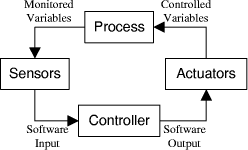
\includegraphics[width=\textwidth]{four_Variables}
    \caption{Vier variabelen model \cite{thompson2000requirements}}
	\label{fig:four_Variables}
\end{figure}

\subsection{Tijd}
In Uppaal wordt tijd globaal op hetzelfde tempo bijgehouden. Tijd wordt in klokken bijgehouden en kan op elk moment worden uitgelezen of gereset. \cite{uppaalsmalltutorial}
\subsection{Guards en invarianten}
Guards zijn condities die op transities worden geplaatst, aan deze condities moet worden voldaan voordat deze transitie mogelijk is.\cite{uppaalsmalltutorial}


guards condities op transities, 

\subsection{Deadlock}

Een deadlock is een situatie waarin er nooit meer verdere state transities mogelijke zijn \cite{uppaalintro}.

\subsection{Zeno gedrag}
Wanneer een model een oneindig aantal transities kan maken in een bepaalde tijd dat wordt er gesproken van zeno gedrag \cite{uppaaltutorialmodelingpatterns} \cite{leine2011zeno}.
\section{Logica}

Dit is een herhaling van eerste jaars logica. Er wordt met modale logica gewerkt, waarbij voor ons vooral de focus ligt op temporale logica, een aantal van de voorbeelden zijn hierop afgesteld.

\subsection{Propositielogica}

Propositie zijn uitspraken die waar of onwaar kunnen zijn. Propositielogica is houdt zich bezig met het redeneren van deze logica.

\subsection{Predicatenlogica} \label{PredicateLogic}

Predicaten zijn statements over de relaties tussen dingen. Deze logica bevat de universele en existentiële kwantoren of respectievelijk '\forall' en '\exists'.

Voorbeelden van deze logica zijn statements zoals: Voor alle appels geld dat ze fruit zijn, of voor alle het fruit geldt dat er uiteindelijk een zal zijn die een appel is.

\subsection{Kwantoren}

In de logica bestaan zogeheten kwantoren. Kwantoren zijn symbolen die relaties tussen variabelen aangeven. Hierboven onder het kopje \nameref{PredicateLogic} zijn al twee kwantoren aangeduid namelijk '\forall' en '\exists'.

\subsection{Dualiteiten}

Een dualiteit is een wanneer een statement die naar voren komt wanneer een andere statement een negatie ondergaat. Als voorbeeld, in modale logica, als de propositie 'voor alle P geld dat deze altijd waar is' een negatie ondergaat dan kunnen wij door dualteit de proposite maken 'voor alle p geld dat deze soms waar is'.

\section{Computation tree logic}

\subsection{De computation tree}

De computatie boom is een model om tijdsgebonden logica te modelleren. \\\\
In dit model bestaan de volgende temporale operatoren:
\begin{itemize}
    \item A Always
    \item E Exists
    \item F Eventually
    \item G Globally
    \item X Next
\end{itemize}
Deze operatoren kunnen worden gecombineerd zoals hieronder is aangetoond.

\subsection{Operator: Always Global (AG)}

Een bepaalde propositie is waar voor elke mogelijke staat in het model.

\subsection{Operator: Exists Global (EG)}

Een staat waarin een bepaalde propositie waar is kan worden bereikt. Maar nadat deze is bereikt zal de propositie niet meer vals kunnen zijn.

\subsection{Operator: Always Eventually (AF)}

Elke tak van het model bevat een staat waarvoor een gegeven propositie waar zal zijn.

\subsection{Operator: Exists Eventually (EF)}

Het is mogelijke dat een bepaalde staat zal worden bereikt waarin de gegeven propositie waar is.

\subsection{Operator: Always Next (AX)}

Een bepaalde staat zal altijd worden opgevolgd door een staat waarvoor een bepaalde propositie waar zal zijn.

\subsection{Operator: Exists Next (EX)}

Een bepaalde staat kan een transitie uitvoeren naar een staat of staten waarvoor een bepaalde propositie waar is.

\subsection{Operator: p U q}

p en q zijn voor dit voorbeeld verzameling. p U q betekent 'alle objecten die tot p of q behoren' alsof p en q samen één grote verzameling vormen, U staat dan ook voor Union.

\subsection{Operator: p R q}

\subsection{Fairness}

Een eis van het systeem dat deze op eerlijke wijze de volgende staat kiest. Het doel hierbij is dat elke state in het systeem uiteindelijk waar zal zijn.

\subsection{Liveness}

Liveliness is the vereiste dat een bepaald doel in het systeem kan worden bereikt. Om dit mogelijk te maken is er Fairness nodig, als een bepaald process immers nooit draait dan kan het zijn dat een bepaald doel niet bereikbaar is \cite{fairnessandliveness}.

\newpage
\subsection{Temp log:}
Sheets:

inleiding w1
state transition diagrams w2
modellen w2
computation tree logic w3


week 1: 
world vs. machine
requirements en specifications |
systems engineering vs. software engineering
4 variablen |
week2:
tijd
guards en invarianten
deadlocks
week3:
logica
temporele logica (ctl)
(Computation tree logic
Linear tree logic
CTL*: combinatie van bovenstaande twee)
//zie dia voor example images van ctl logica
week4:




Wat is een goed model? cite the links from powerpoint, first links describes what the dia explains, deze link wordt ook gebruikt om de eindopdracht te beoordelen, eindverslag moet afweging laten zien wat betreft je keuzes, wat zijn je argumenten?

google scholar "to predict and serve?"

een goed model moet het verschil tussen ruis en echte informatie kunnen aantonen.

uppaal for sharing int below 5 don't use global variables

ebsilon/absilon-delta stelling wiskunde limiet begrip
\newpage
\bibliography{references}
\bibliographystyle{plain}
\end{document}


Onderwerp(en): 
Nucleaire testen op het eiland Bikini Atoll.
vlucht 1951 mode confusion turkish airlines
kannon met dubbele loop, John Gilleland
Tsjernobly 1986
ariane 5 64 bit getal wrong format

Context:
bikini eilanden, bom die 5 megaton hogere yield had dan verwacht. vakkennis was er nog niet wat betreft physika om dit te kunnen voorspellen.